\documentclass[11pt, oneside]{article}   	% use "amsart" instead of "article" for AMSLaTeX format
\usepackage{geometry}                		% See geometry.pdf to learn the layout options. There are lots.
\geometry{letterpaper}                   		% ... or a4paper or a5paper or ... 
%\geometry{landscape}                		% Activate for for rotated page geometry
%\usepackage[parfill]{parskip}    		% Activate to begin paragraphs with an empty line rather than an indent
\usepackage{graphicx}				% Use pdf, png, jpg, or eps� with pdflatex; use eps in DVI mode
								% TeX will automatically convert eps --> pdf in pdflatex		
\usepackage{amssymb}
\usepackage{amsmath}
\usepackage{parskip}
\usepackage{color}

\title{funny coord}
%\author{The Author}
%\section{}
% \subsection*{R code}
\date{}							% Activate to display a given date or no date

\graphicspath{{/Users/telliott_admin/Dropbox/Tex/png/}}

% \begin{center} 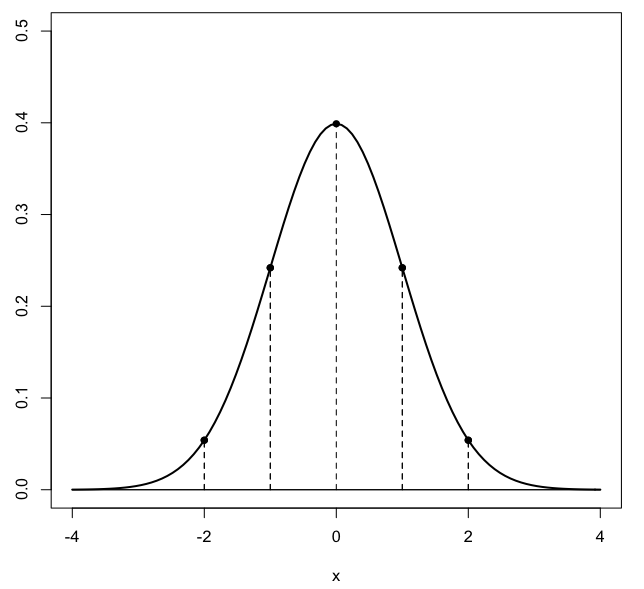
\includegraphics [scale=0.4] {gauss3.png} \end{center}
% \begin{bmatrix} a  &  b \\ c  &  d \end{bmatrix}
% \bigg |_

\begin{document}
\maketitle
\Large
%\noindent

Integrate the unit square in polar coordinates!  Notice the bounds for $r$, the outer limit is $\sqrt{1+ \sin^2 \theta}$.

\[ \iint_R dA = \int_0^{\pi/2} \int_0^{\sqrt{1+\sin^2 \theta}} r \ dr \ d \theta \]
inner integral 
\[ = \frac{1}{2}r^2  \ \bigg|_0^{\sqrt{1+ \sin^2 \theta}} \]
\[ = \frac{1}{2} (1 + \sin^2 \theta ) \]
outer integral
\[ = \int_0^{\pi/2}  \frac{1}{2} (1 + \sin^2 \theta ) \ d \theta \]
Look it up
\[ =  \frac{1}{2} \ [ \ \theta  + \frac{1}{2}(\theta - \frac{1}{2}\sin 2 \theta) \ ] \  \ \bigg|_0^{\pi/2}   \]
The first $\theta$ gives us $\pi/4$ and the rest is
\[ =  \frac{1}{4}(\theta - \frac{1}{2}\sin 2 \theta) \ ] \ \bigg|_0^{\pi/2}  \]
The second $\theta$ gives us $\pi/8$ leaving
\[ = -\frac{1}{8} \sin 2 \theta  \ \bigg|_0^{\pi/2}  \]
which is $0$.
So we have a total of $3/8 \pi$, which is wrong!

\end{document}  